%
% File naacl2019.tex
%
%% Based on the style files for ACL 2018 and NAACL 2018, which were
%% Based on the style files for ACL-2015, with some improvements
%%  taken from the NAACL-2016 style
%% Based on the style files for ACL-2014, which were, in turn,
%% based on ACL-2013, ACL-2012, ACL-2011, ACL-2010, ACL-IJCNLP-2009,
%% EACL-2009, IJCNLP-2008...
%% Based on the style files for EACL 2006 by 
%%e.agirre@ehu.es or Sergi.Balari@uab.es
%% and that of ACL 08 by Joakim Nivre and Noah Smith

\documentclass[11pt,a4paper]{article}
\usepackage[hyperref]{naaclhlt2019}
\usepackage{times}
\usepackage{graphicx}
\usepackage{booktabs}

\usepackage{latexsym}
\usepackage{amsmath}
\usepackage{amssymb}
\usepackage{bm}

\newcommand{\rdep}[1]{\ $\xrightarrow{\text{\tiny #1}}$\ }


\newcommand{\ahcomment}[1]{\textcolor{blue}{[#1 -AH]}}

\usepackage{url}

%\aclfinalcopy % Uncomment this line for the final submission
%\def\aclpaperid{***} %  Enter the acl Paper ID here

%\setlength\titlebox{5cm}
% You can expand the titlebox if you need extra space
% to show all the authors. Please do not make the titlebox
% smaller than 5cm (the original size); we will check this
% in the camera-ready version and ask you to change it back.

%\hypersetup{draft} % THIS IS NEEDED TO GET IT TO COMPILE. Does not like the tables. AH 11/27

\newcommand\BibTeX{B{\sc ib}\TeX}

\DeclareMathOperator*{\argmaxA}{arg\,max} % Jan Hlavacek

% Extractive sentence compression under lexical and length constraints
\title{Transition-based Sentence Compression with Lexical and Length Constraints}

\author{First Author \\
  Affiliation / Address line 1 \\
  Affiliation / Address line 2 \\
  Affiliation / Address line 3 \\
  {\tt email@domain} \\\And
  Second Author \\
  Affiliation / Address line 1 \\
  Affiliation / Address line 2 \\
  Affiliation / Address line 3 \\
  {\tt email@domain} \\}

\date{}

\begin{document}
\maketitle

% \ahcomment{Proposed revision: In this work we present a new, transition-based framework for extractive sentence compression. We use this framework to construct a sentence compression system based on a very simple neural network, which achieves large gains in automatic evaluation measures over previous state-of-the-art approaches. Unlike prior techniques, our method also allows accommodates lexical and length constraints without incurring exponential computational costs. This makes our method better suited to user-facing search applications, where length and lexical constraints are paramount.}

% \ahcomment{note: gurobi pool search mode is turned ON which makes everythign go slower. you should turn this off if you start making arguments about wall clock time}


\begin{abstract}
Traditional approaches to extractive sentence compression seek to reduce the length of a sentence, while retaining the most ``important'' information from the source. But query-focused applications such as document search engines or exploratory search interfaces place additional lexical and length requirements on compression systems. This study introduces a new transition-based, neural compression method which accommodates such requirements by pruning syntactic dependency subtrees.  We show that our technique is more computationally efficient than previous ILP-based approaches, and achieves competitive performance in reconstructing known-good shortenings under constraints.
\end{abstract}

\section{Introduction}

Traditional study of extractive sentence compression seeks to create short, readable compressions which retain the most ``important'' information from source sentences. But query-focused and user-facing applications impose additional requirements on the output of a compression system. Compressions must be short enough to be shown in a user interface and must contain a user's query term, which defines the ``important'' information in the sentence. An example of such a compression is shown in Figure \ref{f:qf}.

This study examines the English-language compression problem with such length and lexical requirements: compressed sentences are (1) required to include a list of query words $q$ and (2) be shorter than or equal in length to a maximum character length, $b \in \mathbb{Z}^{+}$. While older compression methods based on integer linear programming could trivially accommodate such restrictions \cite{clarke2008global,filippova2013overcoming}, recent work has focused on neural network techniques which can often reconstruct gold-standard shortenings \cite{filippova2015sentence}, but which do not give practitioners such control. This makes existing sequence-to-sequence techniques unsuitable for search engines \cite{hearst2009search}, concept map browsers \cite{falke2017graphdocexplore} and new forms of exploratory textual interfaces \cite{marchionini2006exploratory}, where length and lexical constraints are paramount. 

\begin{figure}[htb!]
%\fbox{
%\begin{minipage}{7.6 cm}
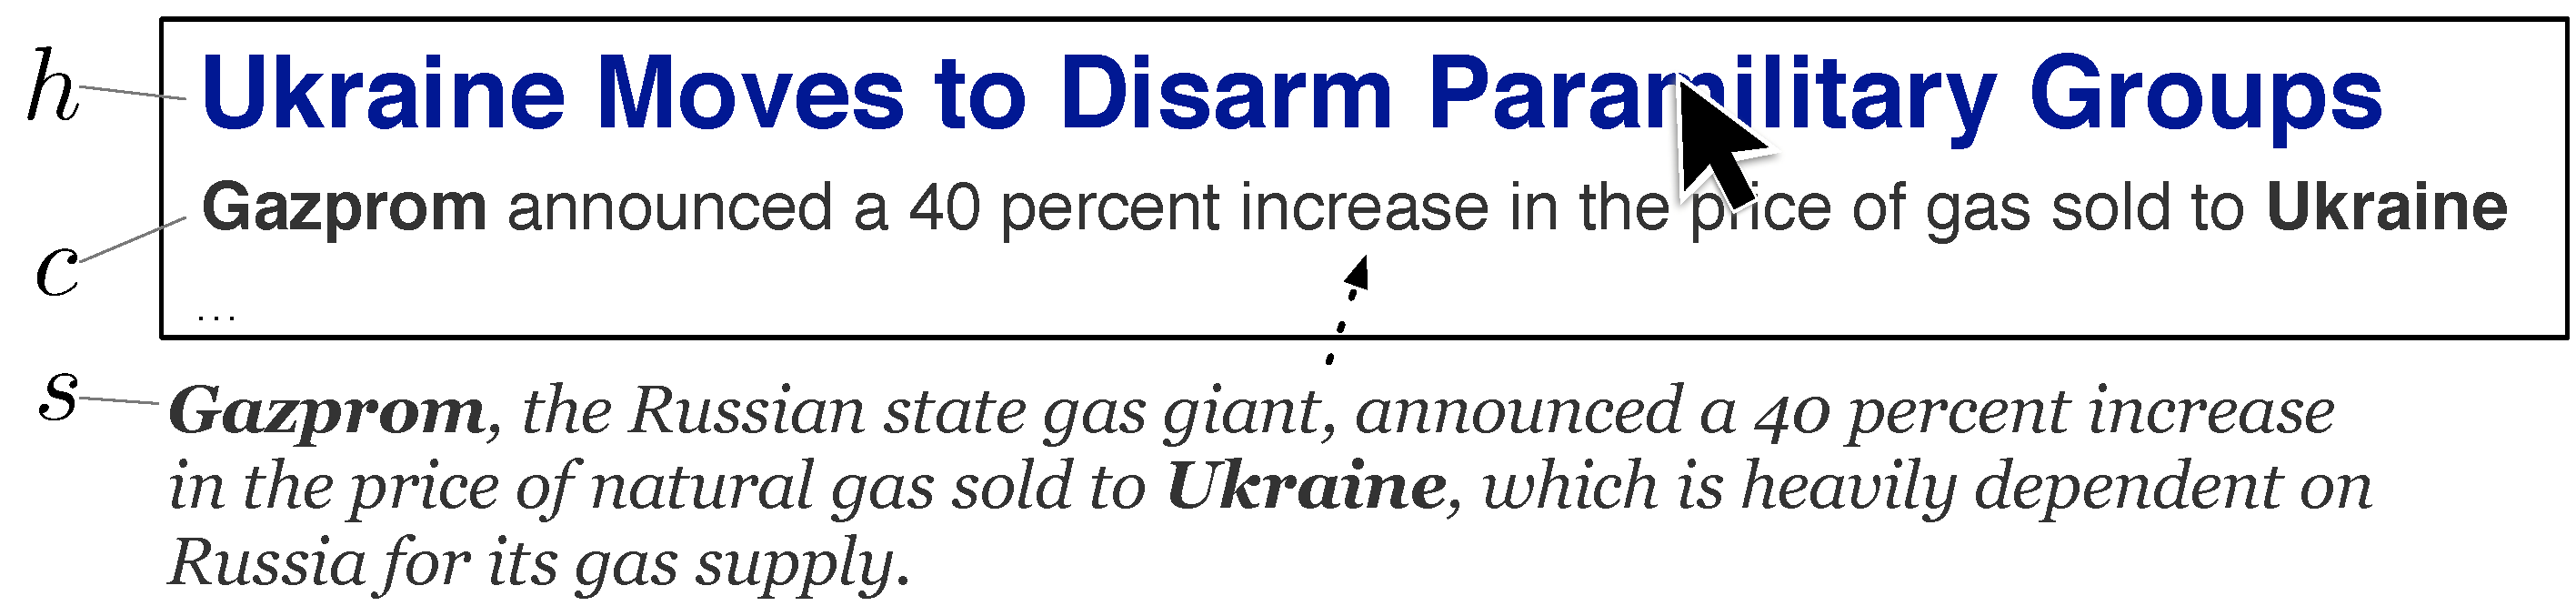
\includegraphics[width=8.5cm]{qf.pdf}
\caption{Search interfaces often require compressions with length and lexical constraints. In this case, a search interface (boxed, top) returns a headline $h$ above a constrained compression $c$, shortened from a sentence $s$ in a query-relevant document (italics, bottom). The constrained compression must contain the users' query terms (bold), and must not exceed 75 characters in length.}
\label{f:qf}
%\end{minipage}
%}
\end{figure}

\begin{table*}[htb!]
\begin{tabular}{lccc}
\textbf{Approach} & \textbf{Worst-case complexity} & \textbf{Constrained}  \\ \hline
LSTM taggers \cite{filippova2015sentence}   & linear              & no         \\   
\textbf{Iterative deletion (this work)}  & \textbf{quadratic}     &      \textbf{yes}   \\
ILP    \cite{filippova2013overcoming,Wang2017CanSH}       &   exponential    & yes      \\
\end{tabular}
\caption{Three algorithms for sentence compression. Linear programming methods \cite{clarke2008global,filippova2013overcoming,Wang2017CanSH} can easily accommodate length and lexical constraints, and can make use of large parallel corpora of sentence--compression pairs. But these methods formulate the compression task as an NP-complete optimization problem (\S\ref{s:ilps}), with worst-case exponential runtime. LSTM taggers \cite{filippova2015sentence} achieve comparable results with a linear runtime, but cannot accommodate length or lexical requirements. This work introduces a supervised, transition-based approach (\S\ref{s:system}) which can be used to compress sentences under lexical and length constraints in quadratic time.} 
\label{t:algos}
\end{table*}


Therefore, in this work, we present a new method for compressing sentences, which efficiently accommodates lexical and length constraints. Our transition-based, stateful compression method is inspired by similar approaches to transition-based dependency parsing \cite{nivre2003,D14-1082}. We compare this supervised, transition-based technique to supervised, ILP-based systems, which also accommodate length and lexical restrictions. We show that our method has lower computational costs while better reconstructing known-good, constrained shortenings, as measured by token-level F1 score. 

\section{Compression and constraints}

This work contrasts traditional ILP-based compression with our novel transition-based framework. We also briefly discuss compression with sequence-to-sequence methods, which do not accommodate length or lexical requirements. Table \ref{t:algos} provides a summary of each approach.

\subsection{Constrained compression with ILPs}\label{s:ilps}

One common approach for shortening sentences formulates compression as an integer linear programming (ILP) task. ILP-based methods assign binary variables to each token in a sentence \cite{clarke2008global} or subtree in a dependency parse \cite{filippova2008dependency}. These variables indicate if the corresponding component included in a compression. Each such sentence component is also assigned a local weight, indicating its worthiness for inclusion in a shortened sentence. Local weights are either learned from direct supervision \cite{filippova2013overcoming,Wang2017CanSH}, or inferred from sources like corpus statistics, importance score metrics and n-gram language models \cite{clarke2008global,filippova2008dependency}.

Such ILP methods represent the overall quality of a compression by summing the local weights of sentence components to compute a global objective score.  The task of identifying the best possible solution to an integer programming objective is a well-known, NP-complete problem, which requires exponential computation in the length of the input sequence. Researchers use off-the-shelf ILP solvers to identify the highest-scoring compression, from among all possible configurations of binary variables (each variable may be set to 0 or 1).

This integer linear programming approach also easily accommodates constrained compression. Researchers will customarily add constraint terms to the ILP objective to enforce hand-build semantic restrictions \cite{clarke2008global} or syntactic requirements \cite{filippova2008dependency}. Adding additional length or lexical requirements to ILPs is trivial: practitioners must specify that optimal solutions must be shorter than some character budget, and must specify that binary variables marking inclusion of particular words must be set to 1. 

In practice, translating a sentence compression objective into an integer linear program is a challenging and error-prone programming task, dependent on black-box optimization techniques. These engineering difficulties are a disadvantage of ILPs.

\subsection{Transition-based constrained compression}

In this work, we present an alternative, transition-based method for shortening sentences under lexical and length constraints, inspired by transition-based parsing techniques \cite{Earley1970AnEC,nivre2003}. Our method compresses a sentence over $N$ time steps, by adding and removing $N$ different subtrees from a dependency parse, one after another. Our stateful approach recalls early solutions to the sentence compression problem \cite{Jing2000SentenceRF,Knight2000StatisticsBasedS}, which also shortened sentences by executing grammatically-motivated operations on syntax trees. We present the formal details in Section \ref{s:system}. 

Like ILP-based methods, transition-based approaches can easily accommodate lexical and length restrictions. At a high-level, such methods need to add subtrees which contain query terms and remove subtrees which do not contain query terms, until identifying a compression which satisfies the length constraint. However, we show that our transition-based method has a lower computational cost (\S\ref{s:costs}), while achieving better performance than the leading, supervised ILP technique \cite{filippova2013overcoming}.

\begin{table*}[]
\centering
\begin{tabular}{llp{70mm}}
\textbf{Operation} &             \textbf{Definition}                                                    &      \textbf{Description}    \\ \hline
\textsc{Start}      & START $\Rightarrow ( V=\emptyset,  B=[v_1, v_2 ... v_n])$ & Initialize the buffer with the vertexes in the original sentence $s$, arranged breadth-first \\ \hline
\textsc{Prune}              & $(V, [v|B]), v \in V,  \Rightarrow (V \setminus  T(v), B)$ & Remove the subtree rooted at $v$ in $s$ from $V$ \\  
$\textsc{Insert}$             & $(V, [v|B]), v \notin V, \Rightarrow (V \cup T(v), B)$ & Insert the subtree rooted at $v$ in $s$ into $V$  \\ \hline
\textsc{NoPrune}           & $(V, [v|B]), v \in V, \Rightarrow (V, B)$ & Don't remove the subtree rooted at $v$ from $V$  \\ 
\textsc{NoInsert}          &       $(V, [v|B]), v \notin V, \Rightarrow (V, B)$ &   Don't insert the subtree rooted at $v$ into $V$    \\ \hline
\textsc{Stop}             & $ (V, B=[]) \Rightarrow$ STOP & Compression ends when the buffer is empty \\                                               
\end{tabular}
\caption{A transition-based sentence compression system with a \textsc{Prune} and \textsc{Insert} operation. The state of the compression system is a tuple $(V, B)$, where $B$ is an ordered buffer of tokens and $[v|B]$ indicates that $v$ is at the head of the buffer. $V$ is a subset of vertexes from the original sentence $s$. $T(v)$ denotes the subtree rooted at $v$ in the original sentence. The \textsc{Prune} operation removes all tokens in $T(v)$ from $V$. The \textsc{Insert} operation adds all vertexes from $T(v)$ into $V$. If the compression system executes a \textsc{NoPrune} or \textsc{NoInsert}, $v$ is removed from the head of the buffer and $V$ is not modified. $B$ is initialized with all tokens from $s$ (arranged in breadth-first order) at the \textsc{Start} of compression. Once the buffer is empty, compression will \textsc{Stop} and all vertexes in $V$ are linearized in their original order. These operations can fully reconstruct all shortenings in a standard compression corpus \cite{filippova2013overcoming}. The appendix presents a complete, worked example.}
\label{t:ops}
\end{table*}

\subsection{Unconstrained compression with LSTMs}

We contrast transition-based compression and integer programming approaches with LSTM taggers for the compression task \cite{filippova2015sentence}. Such taggers achieve state-of-the-art scores on extractive sentence compression, using sequence-to-sequence methods which label tokens with a 1 or a 0 indicating if the token should be included in a summary. This approach is linear in the token length of a the input sequence. However, at this time, LSTM taggers are unsuitable for query-focused applications because such methods cannot enforce lexical or length requirements. This limitation might be reexamined in future work, using new work on constrained generation \cite{N18-1119,aaimh}.

\section{Transition-based sentence compression}\label{s:system}

In this work, we present a new transition-based sentence compression system, inspired by similar approaches in transition-based parsing \cite{nivre2003,D14-1082}. Our compression system maintains a state, modified by a small set of operations. We formally describe the system (\S\ref{s:formal}), present a method for generating oracle paths to gold standard shortenings (\S\ref{s:oracle}), and then detail a computational model of oracle compression (\S\ref{s:modeling}). We then demonstrate and evaluate a method which uses this model for constrained compression (\S\ref{s:transition}), and analyze its computational costs (\S\ref{s:costs}).

\subsection{Formal description}\label{s:formal}

Our transition-based sentence compression system shortens a sentence $s$ by executing a sequence of operations. Each operation modifies the state, denoted $(V,[v|B])$, where $V$ is a subset of tokens from $s$, and $B$ is an ordered buffer of tokens from $s$ headed by the token $v$. In defining each operation, we use the notation $T(v)$ to refer to the subtree headed by $v$ in the unchanging, precomputed dependency parse of $s$.

We define four principal operations, which reference the vertex $v$ at the head of the buffer, $[v|B]$. The operation \textbf{\textsc{Prune}} removes all vertexes in $T(v)$ from $V$. The operation \textbf{\textsc{Insert}} adds $T(v)$ into $V$. Executing a \textsc{Prune} or \textsc{Insert} also pops the token $v$ from the head of the buffer. The compression system can also execute the operations \textbf{\textsc{NoPrune}} and \textbf{\textsc{NoInsert}}, which pop $v$ from the buffer without inserting or pruning $T(v)$. 

To generate a compression, we first execute the $\textbf{\textsc{Start}}$ operation which sets $V=\emptyset$ and defines $B=[v_1, v_2 ... v_{|s|}]$, where $v_1, v_2 ... v_{|s|}$ are the tokens in $s$, arranged breadth-first, and $|s|$ is the token length of the original sentence. After the buffer is empty, we execute a $\textbf{\textsc{Stop}}$ operation and all tokens in $V$ are linearized in their original order to return a shortened sentence. Table \ref{t:ops} formally defines all operations. The appendix also includes a complete, worked example. 

In our transition-based compressor, only some operations are valid for some configurations of the state. If $v \notin V$, then $\textsc{Prune}$ is not valid as $T(v)$ cannot be removed from $V$. Similarly, if $v \in V$, then $\textsc{Insert}$ is not valid as $T(v)$ cannot be added to $V$. Table \ref{t:ops} includes these preconditions in the definition of each operation.

\begin{figure*}[htb!]
\centering
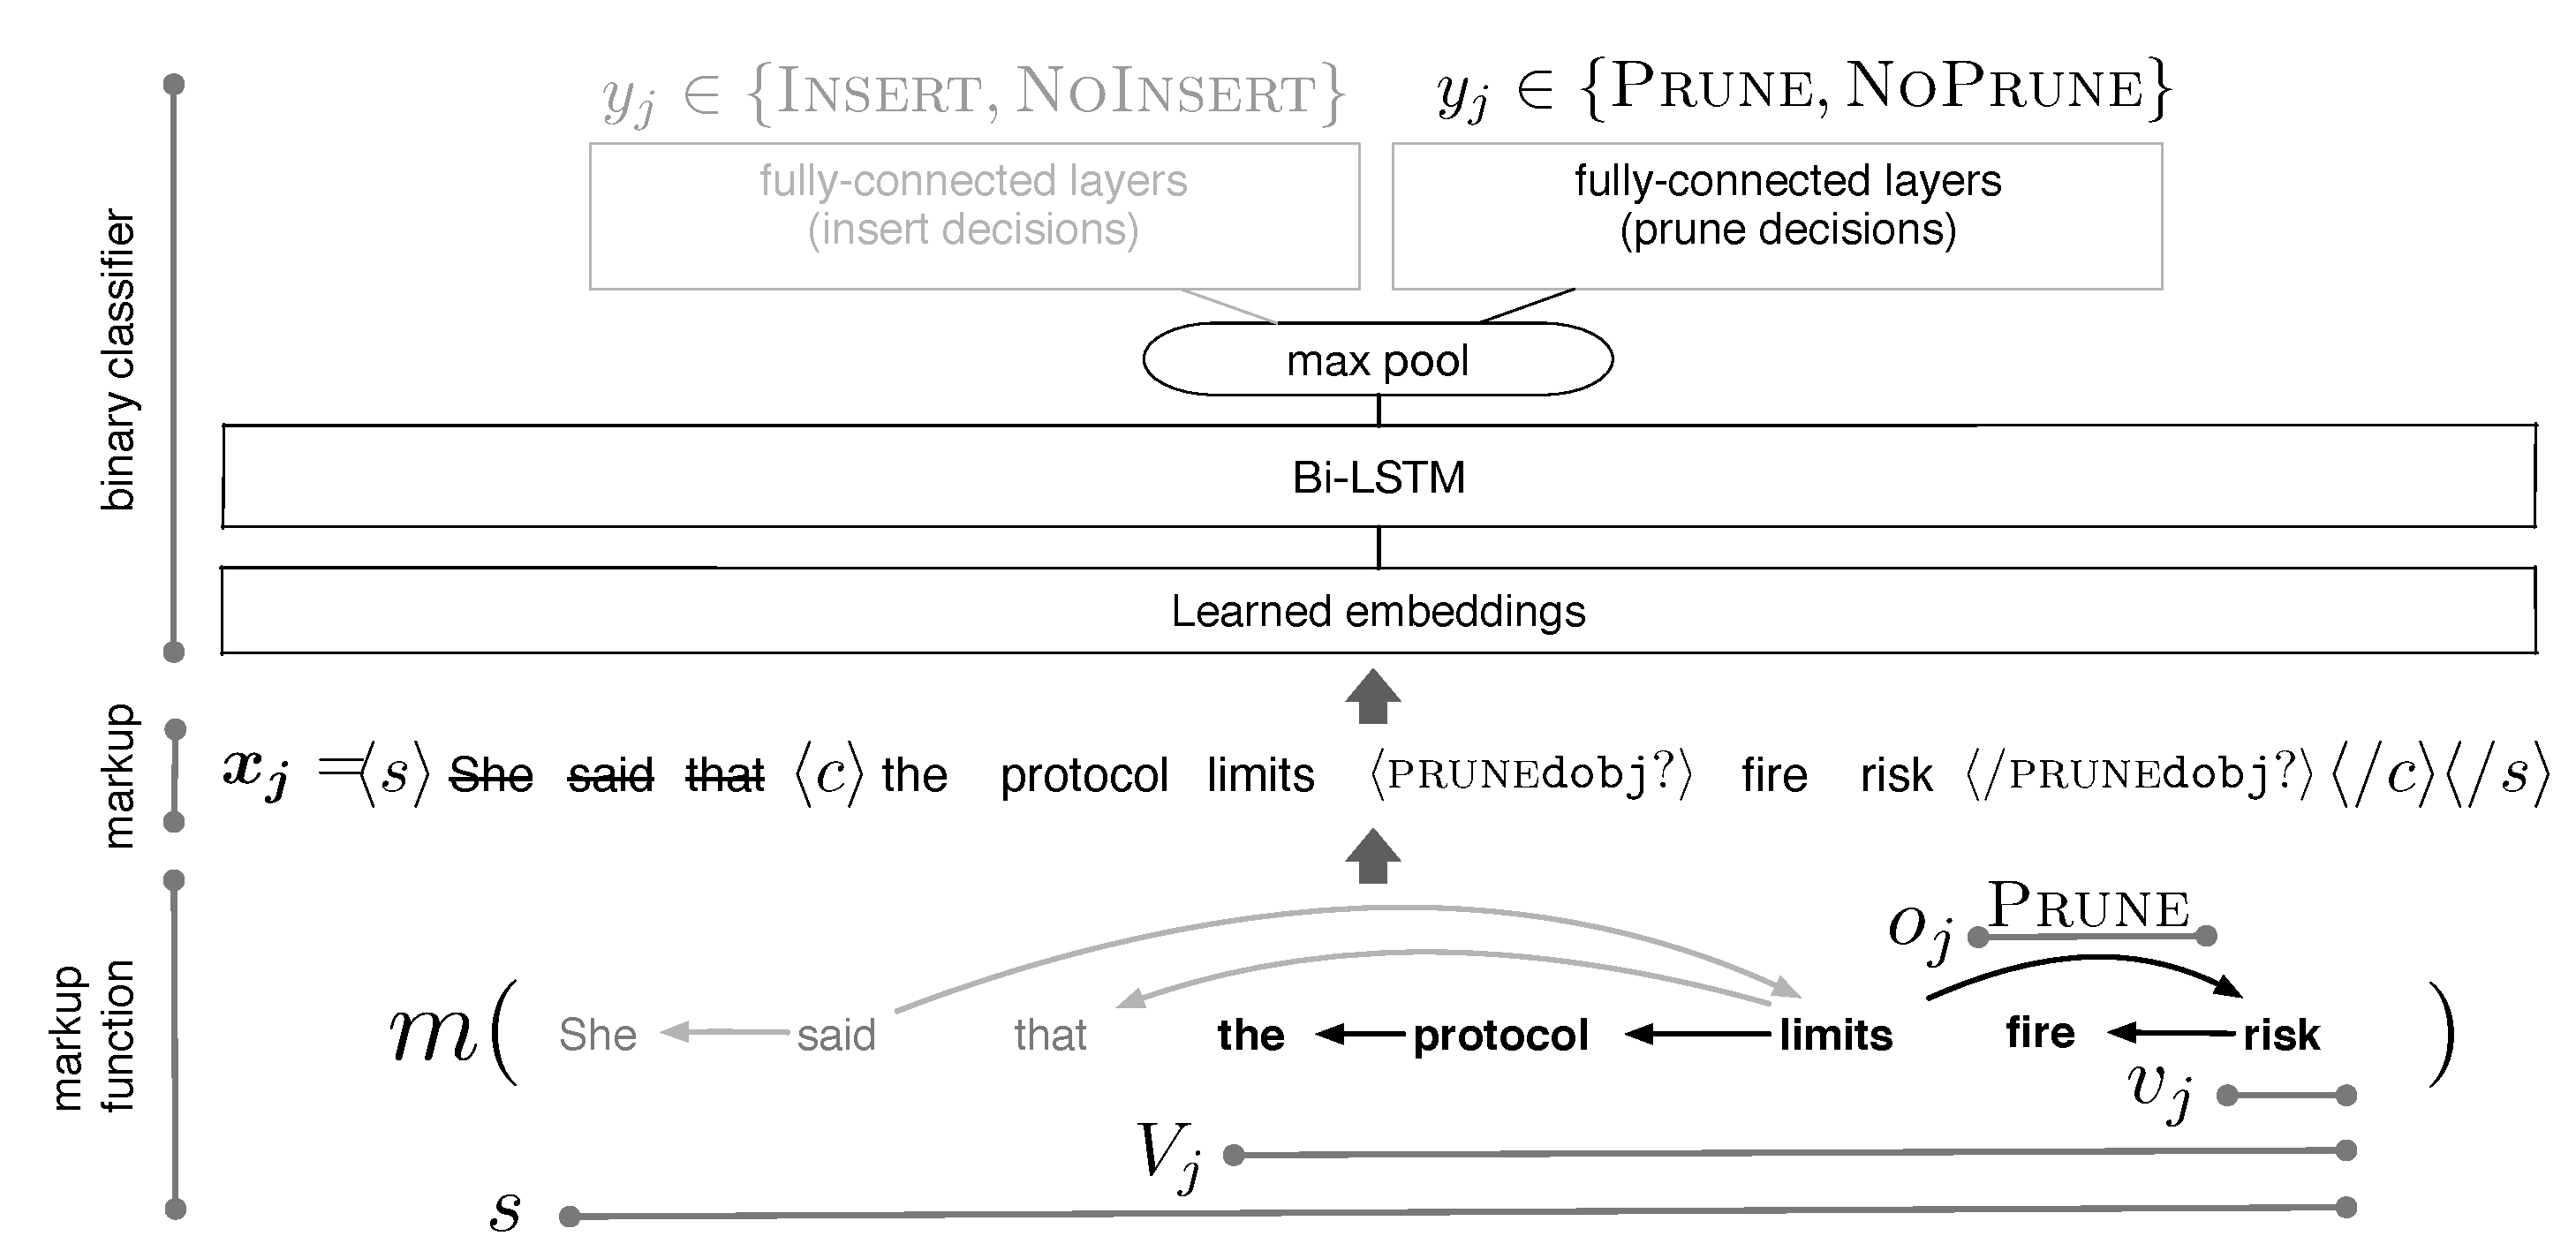
\includegraphics[width=.85\textwidth]{example.pdf}
\caption{Our neural classifier, which learns to make a binary decision based on the markup, $\bm{x}$ (\S\ref{s:modeling}). The model uses a shared Bi-LSTM and max pooling layer, along with fully-connected layers responsible for binary \textsc{Prune} decisions, and fully-connected layers responsible for \textsc{Insert} decisions. The appropriate task for the LSTM (i.e. prune decision vs. insert decision) is always clear from context (\S\ref{s:oracle}). The markup $m(V_j,v,o,s)=\bm{x}$ ``shows'' the LSTM what a proposed change to the state of the compression system would ``look'' like if the operation proposal $o$ were to be carried out. At each timestep, LSTM must decide if the stateful compression system should accept the operation proposal, $o \in \{\textsc{Prune}, \textsc{Insert}\}$. In this case, $s$ is ``She said that the protocol limits fire risk'' and $V_j$ is ``the protocol limits fire risk''.  The LSTM must decide if the compression system should execute $o$= \textsc{Prune} on the subtree headed at $v$ = \textit{risk}, governed by a $\texttt{dobj}$ edge in the parse. }
\label{f:example}
\end{figure*}

\subsection{Oracle paths}\label{s:oracle}

We identified the operations in our compression system empirically: we found that for all compressions in a large, standard corpus \cite{filippova2013overcoming} there exists an oracle path of at most $|s|$ operations which can fully reconstruct the shortened sentence, where $|s|$ denotes the token length of the original sentence.

We identify the oracle path by executing  a sequence of operations. Let $(V_j, v_j | B)$ denote the state at timestep $j$. The oracle operation at step $j$ is unambiguously determined by $c_g$, the vertexes in the gold compression. For instance, if $v_j \in V_j$ but $v_j \notin c_g$, then the oracle must execute \textsc{Prune}. This is because $B$ is arranged breadth-first, so our system can only remove $v_j$ at timesteps $j^{\prime} \leq j$. If the vertex is not pruned at timestep $j$, the system will never have an opportunity to remove it and will never recover $c_g$. Similarly, if $v_j \in c_g \cap V$ then the oracle operation at timestep $j$ must be $\textsc{NoPrune}$. This is because if the system were to prune $v_j$ at timestep $j$, it will not have the opportunity to reinsert the vertex again at a later timestep. We use analogous reasoning to identify oracle $\textsc{Insert}$ and $\textsc{NoInsert}$ operations. By executing each oracle operation in sequence, we compress $s$ to $c_g$ and identify the oracle path.

Because it is only possible to prune $v_j$ if $v_j \in V$, and only possible to insert $v_j$ if $v_j \notin V$ (\S\ref{s:formal}), we interpret the oracle path as a sequence of binary decisions. If $v \in V$, the compression system must decide to execute $\textsc{Prune}$ or $\textsc{NoPrune}$. If $v \notin V$, it must decide to execute $\textsc{Insert}$ or $\textsc{NoInsert}$. We use this interpretation of the oracle path during modeling.

\subsection{Modeling}\label{s:modeling}

In our framework (\S\ref{s:oracle}), oracle compression is a series of binary decisions. At each step $j$ the oracle must decide to execute (or not execute) some operation proposal, $o \in \{\textsc{Prune}, \textsc{Insert}\}$. We train an LSTM to predict the binary oracle decision $y \in \{0,1\}$ based on the state of the compression system and the operation proposal, where $y=1$ indicates that the compression system accepts the proposal (e.g. executes $\textsc{Prune}$) and $y=0$ indicates that the compression system does not accept the proposal (e.g. executes $\textsc{NoPrune}$).

To train the LSTM, we deterministically encode both the state of the compression system and the operation proposal into a sequence of input symbols $\bm{x}$, called the markup. The LSTM predicts $p(y=1 | \bm{x})$, the probability of a binary oracle decision, given the markup. 

The markup is the deterministic (rather than learned) output of a function $\bm{x}=m(V_j,v,o,s)$, which inserts three sets of matched, inline bracket symbols into $s$, the original sequence of tokens in the sentence. The bracket symbols represent the following information:

\begin{enumerate}
\item{The start and end of the original, uncompressed sentence $s$. This set of bracket symbols are shown with $\langle s \rangle$ and $\langle / s \rangle$ in Figure \ref{f:example}.}
\item{The start and end of \textsc{Max}($V_{j+1}, V_{j}$) within $s$ where, \textsc{Max} selects the largest set by cardinality and where $V_{j+1}$ is all tokens which would be in $V$ at step $j+1$, if the system were to execute operation $o$ at timestep $j$. If $o=\textsc{Prune}$ then $V_{j+1}$ will be smaller than $V$ and the bracket symbols will show the extent of the current $V_j$. If $o=\textsc{Insert}$, then $V_{j+1}$ will be larger than $V$ and the bracket symbols will show the extent of the compression which would result if the tokens were to be inserted at timestep $j$. This set of bracket symbols are shown with $\langle c \rangle$ and $\langle / c \rangle$ in Figure \ref{f:example}.\footnote{In some cases, some of the tokens in the span from $\langle c \rangle$ to $\langle /c \rangle$ might not be in $V_{j + 1}$. This is possible, for instance, at time $j+1$ if a compression system pruned a modifier from the middle of a span of tokens at step $j$.}}
\item{The start and end of $T(v)$, defined previously (\S\ref{s:formal}) as the tokens in the subtree which would be pruned or inserted by the operation proposal $o$. This set of bracket symbols, called \textit{subtree tags}, have a more complex structure which encodes $(i)$ the type of the operation proposal $(ii)$ the syntactic role of $T(v)$ within $s$. Figure \ref{f:example} shows the subtree tags $\langle \textsc{Prune} \texttt{dobj} ? \rangle$ and $\langle / \textsc{Prune} \texttt{dobj} ? \rangle$. Details of the structure of subtree tags are provided in the appendix (\S\ref{s:subtree})}
\end{enumerate}

The markup function also includes information about which individual tokens from $s$ are in (or not in) the current compression $V_j$. The function concatenates special indicator tags to all tokens $t_i \in \{s\} \setminus V$, where $\{s\}$ denotes the unordered set of tokens from the ordered sequence $s$. (These indicator tags are denoted with strikethrough text in Figure \ref{f:example}.) 

Including the three sets of inline bracket tags, along with the indicator tags, allows the LSTM to model the relationship between $(a)$ the tokens to be pruned or inserted, $(b)$ the current compression, $(c)$ the operation proposal, and $(d)$ the original sentence $s$. Prior work shows that LSTMs appear capable of modeling bracketing within a sentence \cite{Vinyals2015GrammarAA,karpathy,Aharoni2017TowardsSN}.

Our architecture (Figure \ref{f:example}) follows recent work on LSTM classification for sentence-level tasks \cite{D17-1070}. Specifically, we predict binary, oracle operations using a Bi-LSTM layer, a max pooling layer, and two separate sequences of fully-connected layers: one for \textsc{Prune} vs. \textsc{NoPrune} decisions, and one for \textsc{Insert} vs. \textsc{NoInsert} decisions. We interpret the shared Bi-LSTM layer as learning deep features from the markup \textbf{x}, and each sequence of fully-connected layers as using those features to perform a different kind of binary classification.

%\footnote{The symbols $\langle {o \cdot d} \rangle$ and $\langle / {o \cdot d} \rangle$  allow us to encode some aspects of syntax trees using a vanilla LSTM , without the added complexities of explicitly encoding nested structures into the architecture of the network \cite{Tai2015ImprovedSR,Dyer2016RecurrentNN}.} }

%It lets the LSTM reason about the relationship between the to-prune/insert span, versus the rest of the sentence, by using inline start/end markup symbols. This is motivated by prior work showing that LSTMs are good at modeling inline bracketing within a sentence (CITE: the "parsing as foreign language" paper, and maybe a "LSTMs learn paren balancing" paper, maybe Karpathy or that newer Goldberg one)

 %$(i)$ the first and last  $V_{j + 1}$, if the operation were to be ex

%In this section, we refer to all tokens in $V_j$ as the compression, $c_j$.

% about if these tokens are included or not included in t

%``shows'' the model what a compressed sentence would ``look'' like if the compression system were to execute the operation $o$ given the state $(V, [v|B])$. In the case of insert operations, this means that the markup ``shows'' what the resulting compression would be, if the subtree $T(v)$ were to be copied into $V$. In the case of prune operations, this means that the function ``shows'' what the compression would be if $T(v)$ were to be removed from $V$.

\subsection{Training}

We use a large corpus of sentence--compression pairs \cite{filippova2013overcoming} to define a set of 8 million tuples $\{(\bm{x}_j, y_j) \}_{j=1}^{K}$, where $\bm{x}$ is the markup reflecting some configuration of the compression system at some step $j$ on some oracle path and $y_j \in \{0,1\}$ is a binary variable indicating the oracle choice at timestep $j$.

We initialize with GloVe embeddings \cite{pennington2014glove} and train using weighted cross entropy loss with Adam \cite{Kingma2014AdamAM}. (The appendix details class weighting procedures). Word vectors are updated during training. We weight the cost function in proportion to the prevalence of each class in our training set. We train for 20 epochs, with early stopping if validation accuracy does not improve within 2 epochs.

Our model includes several hyperparameters including: the width of the max pooling layer, the learning rate, the Adam weight decay setting, the activation function, the dropout rate in the fully-connected components and the dimensionality of input embeddings. The final parameters are included in a table in the appendix. We tuned parameters by first searching coarsely and at random over the parameter space \cite{Bergstra2012RandomSF}; and then searching finely and at random over smaller regions of the parameter space which achieve high decision-level accuracy. Our best model achieves a validation accuracy of 0.945\% on a set of 100,000 held-out oracle operations in its highest-performing epoch. We use the learned parameters from this epoch in subsequent compression experiments. We implement with AllenNLP 0.7.1 \cite{Gardner2017AllenNLP}.

\section{Experiment: automatic evaluation of constrained compression}\label{s:autoeval}

We use a large, standard dataset of sentence--compression pairs from \citet{filippova2013overcoming} to evaluate different approaches to length and lexically constrained compression. Using the dataset in this manner requires reinterpreting gold standard data, which does not specify either a query or length constraint. After re-tokenizing, parsing and tagging NER spans from the original dataset with Stanford CoreNLP 3.8.0 \cite{corenlp}, we define all NER tokens\footnote{We use a standard 3-class definition of NER; for our purposes, entities are people, locations or organizations. We exclude sentences from the dataset which do not include NER in the compression.} which lie within the gold compression as the list of query tokens, $q$. We also define the character length of the gold-standard compression as the character budget, $b$. This interpretation allows us to redefine the corpus of $(s,c)$ pairs as a corpus of 4-tuples $(q,s,b,c)$, where $q$ is the query, $s$ is the original sentence, $b$ is the character budget and $c$ is some known-good compression which satisfies the length and lexical constraints. 

\begin{table}[]
\begin{tabular}{ll}
\centering
Approach & Constrained F1  \\ \hline
Query terms only {\small (lower bound)} & 0.384    \\
Supervised ILP  &  0.854          \\
 \textbf{Iterative deletion} &  \textbf{0.875}    \\
\end{tabular}
\caption{The F1 score for our iterative deletion approach to length and lexically constrained sentence compression, along with the F1 score for our reimplementation of a traditional ILP-based approach \cite{filippova2013overcoming}. The difference between the methods is statistically significant. Selecting only query terms for a compression achieves an F1 = 0.384, which is the lower bound for this task.}
\label{t:results}
\end{table}


We then use token-level F1, to measure how well an ILP-based method (\S\ref{s:ilp}) and a transition-based method (\S\ref{s:transition}) method can reconstruct each known-good compression $c$, given the sentence $s$ and the constraints $q$ and $b$. Token-level F1 is the standard automatic evaluation metric for the sentence compression task. Our method better reconstructs known-good compressions. We show results for each in Table \ref{t:results}. We evaluate the significance of the difference in scores with bootstrap sampling  \cite{D12-1091}; the difference is significant {\tiny $(p < 10^{-3})$}.

We also consider how to apply readability and informativeness evaluations to constrained compression (\S\ref{s:readabilityinformativeness}). We describe each method in the following sections.

\subsection{Implementation: transition-based compression}\label{s:transition}

Our model of transition-based sentence compression (\S\ref{s:modeling}) predicts the oracle operation $y$, given the state $(V,[v|B])$. There are many possible ways to use $p(y=1| \bm{x})$ in a query-focused and length-constrained compression system. In this work, we use a simple, greedy \textbf{iterative deletion} technique: at each step $j$ we \textsc{Prune} the subtree rooted at 

$$\argmaxA_{v \in V,q\not\in T(v)}   p(y = 1 | \bm{x})$$

\noindent where $\bm{x}$ is the markup and $y$ is the binary decision to perform a \textsc{Prune} or \textsc{NoPrune} operation (\S\ref{s:modeling}). We continue pruning subtrees until the length of the linearized tokens in $V$ is less than $b$, in which case we stop compression. 

We initialize $(V, [v|B])$ with the smallest subtree from the dependency parse of $s$ which is (1) rooted at a verb and (2) contains all of the tokens in $q$. For roughly two-thirds of sentences $V$ is simply equal to all tokens in the original sentence. In the remaining cases, all tokens in $q$ are contained in some sub-clause of the sentence; the compression is formed by shortening this subclause, instead of shortening the whole sentence. In more than 95\% of sentences, the compression system must make additional \textsc{Prune} decisions after initializing with the smallest subtree

This method is computationally simpler than ILP-based techniques. In the worst case, an iterative deletion method incurs quadratic cost, but in practice costs are linear (\S\ref{s:empiricalcost}).

\subsection{Implementation: ILP-based compression}\label{s:ilp}

We compare our transition-based compression system to a state-of-the-art ILP-based method, presented in \citet{filippova2013overcoming}. To our knowledge, a public implementation of this method does not exist. We reimplement the structured perceptron approach from scratch, achieving a token-level F1 score of  0.712 on the standard compression task. \ahcomment{Revisit. Need for standard task.} % TODO: where number from?

The F1 score in our reimplementation is lower than the than the result reported by the original authors. There are some important differences between our implementation and \citet{filippova2013overcoming}, which arise in part because we use Universal Dependencies (v1) instead of the older dependency system employed in prior work. We describe these differences in detail in the appendix.

\ahcomment{talk about why this task is in certain ways easier. mention the compression rate.
Argue ILPs are hard to program. SLOR not from LCL}

\ahcomment{Comment on why scores are higher for modified task}

\subsection{Readability and importance}\label{s:readabilityinformativeness}

Researchers often use human judgements of \textit{readability} and \textit{importance} to evaluate extractive sentence compression techniques \cite{Knight2000StatisticsBasedS,clarke2008global,filippova2015sentence}. 

However, traditional importance judgements are inappropriate for evaluating constrained compression. In a traditional importance evaluation, humans judge the degree to which a compression retains the most ``important'' information from a source sentence. However, in our constrained compression setting, a user's query determines the ``important'' information from the source. By definition, constrained compression must obey user-defined, importance requirements.
 
As a check on the readability of the compressions produced by each system, we use the automated SLOR metric \cite{lau2015unsupervised} which has been shown to correlate with human judgements of grammatical acceptability, both in general settings and for sentence compression tasks \cite{kannConl}. SLOR normalizes the probability of a token sequence assigned from a language model, by adjusting for both the probability of the individual unigrams in the sentence and for the sentence length.\footnote{Longer sentences are always less probable than shorter sentences; rarer words make a sequence less probable.} The appendix contains additional details of our implementation of SLOR. Our iterative deletion technique achieves a test-time SLOR score of 0.906. The ILP-based approach achieves a SLOR score of 0.876. This automated metric suggests that each method returns roughly equally readable compressions.

\section{Computational costs of transition-based compression}\label{s:costs}

ILP-based approaches to sentence compression formalize the task as a linear programming optimization task, a well-known NP-complete problem with exponential worst-case complexity (\S\ref{s:ilps}). One advantage of our transition-based framework is that it can perform query-focused, budget-constrained compression in worst-case quadratic time. 

We define one unit of computational cost to be the computation required to evaluate one subtree for possible pruning. This cost scales with the token length of the sentence: the more tokens in a sentence, the more subtrees must be considered for deletion.  %One unit of computational cost i i.e. the cost of computing $p(y=1 | \bm{x})$. 

In the worst-case, our method will prune one singleton subtree (i.e. a subtree with one vertex) at each of the $N$ timesteps during compression.\footnote{Intuitively, pruning in this manner would remove a leaf from the (modified) parse tree at each timestep.} If a dependency parse of $s$ contains $|s|$ original vertexes, and $|s_i|$ refers to the token length of the remaining sentence at timestep $i$, then the iterative deletion method requires at most ${\sum_{i = 0}^{|s|} |s_i | = O(|s|^2)}$ possible operations, where it is always the case that $|s_{i + 1}| = |s_{i}|  - 1$ because one token is removed at each step. (This analysis ignores the effect of query and budget constraints on worst-case complexity.)

\subsection{Empirical costs of transition-based compression}\label{s:empiricalcost}

The theoretical worst-case is a poor representation of the empirical costs of our iterative deletion algorithm. In the worst-case, iterative deletion only prunes one vertex from a singleton subtree at each timestep. But in practice, the method often prunes large subtrees which remove many vertexes in a single step. 

%Similarly, in the worst-case, the algorithm must shorten a sentence to match an arbitrarily small character budget, but in practice character budgets will be set to reasonable lengths for shortened English sentences. Finally, in the worst case, $q$ will be empty (i.e. no lexical constraints are specified, so all operations must be considered at each timestep), but in practice practitioners using our query-focused method will likely specify at least one query term which must be included in shortened sentences. 

We therefore measure the empirical costs of our algorithm during the experiment described in Section \ref{s:autoeval}. We count the total number of vertexes considered for possible pruning during the actual compression process, for each sentence in the experiment. We also compute the total number of such operations during an actual, worst-case run of the algorithm. (In a worst case run, only a single token\footnote{Tokens will have different character lengths. We choose the single vertex for removal at random, from among all pruneable singleton subtrees.} is removed at each timestep, without removing query tokens, until the character budget is satisfied.) 

We find that while iterative deletion is polynomial in the worst case (\S\ref{s:costs}), in practice the computational cost scales linearly in the token length of the input sentence (Figure \ref{f:example}). The observed worst case appears to obey the theoretical upper bound of $O(|s|^2)$ operations.

\begin{figure}[htb!]
\centering
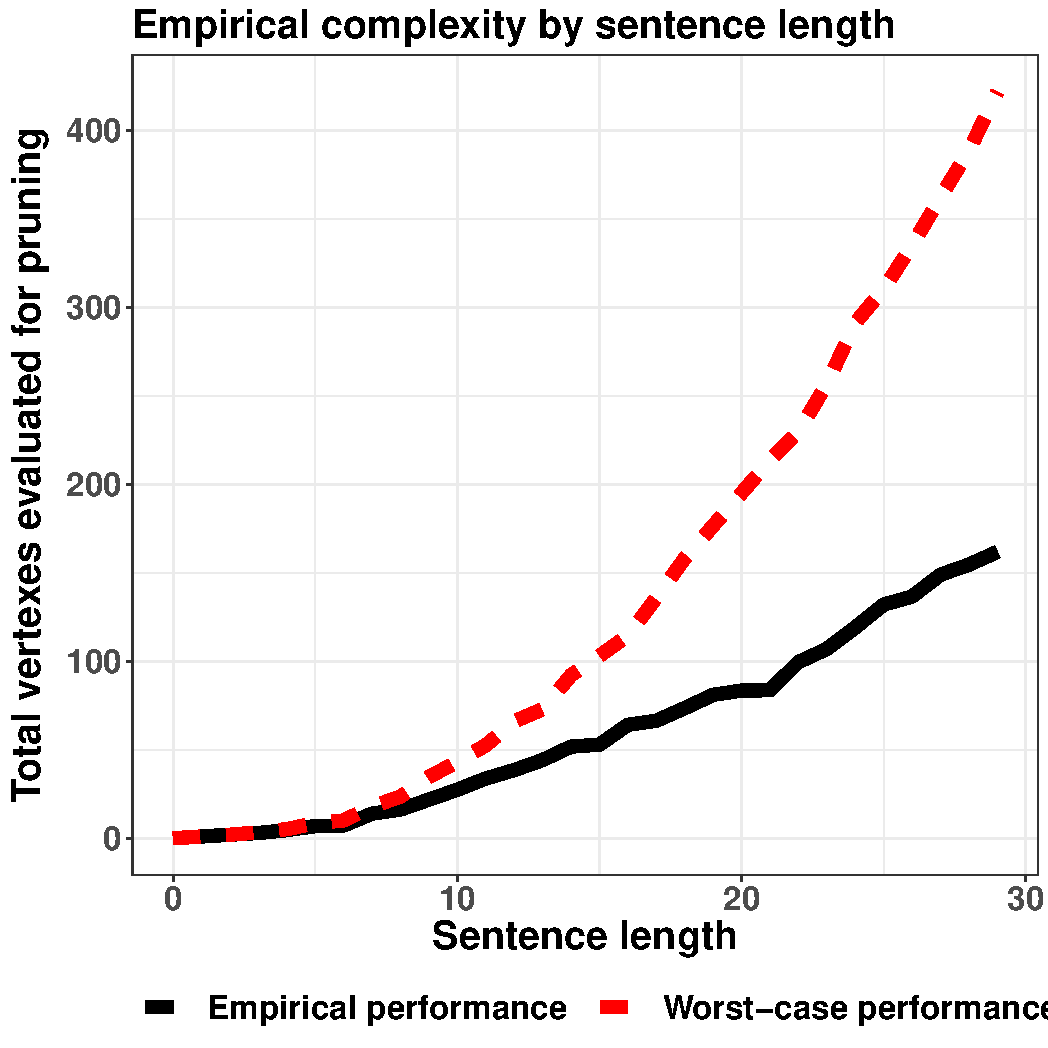
\includegraphics[width=.5\textwidth]{observed.pdf}
\caption{Mean observed operations in a worst case run vs. mean observed operations in an average run of the iterative deletion algorithm, at different sentence lengths. In the worst case (top), iterative deletion is polynomial in the token length of the input sentence (\S\ref{s:costs}). In practice (bottom), empirical costs scale linearly for constrained compression (\S\ref{s:empiricalcost}). The observed worst case appears to observe the theoretical upper bound of $O(|s|^2)$ operations.}
\label{f:example}
\end{figure}

%\subsection{Reducing computational complexity with syntax}

%\ahcomment{Possibly, redo this argument but using the Fillipova/Altun dataset rather than the Brian Dillon dataset. Cut section if not enough time or space.}

%In Section \ref{s:empiricalcost}, we show that the theoretical worst case performance of iterative deletion is a poor representation of the algorithm's empirical performance. In this section, we examine the substantial gap between the mathematical description of the iterative deletion algorithm and the linguistic properties of English syntax. While in principle any vertex may be pruned from a syntax tree, in practice coherent english sentences will require verbs and subjects. Similarly, while in principle any collection of subtrees is a plausible compression, in practice coordinated English phrases must be joined with a conjunction, and prepositions (almost always) cannot be removed from the start of an English prepositional phrase. \ahcomment{look at some deps which are never pruned in FA}

\section{Applications and related work}

Traditional study of sentence compression is motivated by text summarization techniques that create synopses by selecting and (sometimes) shortening sentences \cite{Knight2000StatisticsBasedS,vanderwende2007beyond,martins2009summarization}. 
In these settings, it is important for compressions to retain ``important'' information from source sentences because they must stand-in for longer sentences within summaries.

Our concern with constrained compression is better suited to search applications in which user queries define important information in documents, often shown on a search engine results page \cite{tombros1998advantages,Metzler2008MachineLS}. %Our length and lexically-constrained compressions could be used in information retrieval systems that summarize search results using query-biased snippets on a search engine results page. Often, such snippets must contain query terms, as in Figure \ref{f:qf}. 
Apache Lucene 7.5.0, the leading open source search engine, does not perform sentence compression in generating snippets using its default Fragmenter, Highlighter and Scorer modules.\footnote{https://lucene.apache.org/core/documentation.html} Avoiding grammatical disfluencies in snippets using sentence compression methods could be used to make search engine results more readable \cite{kanungo2009predicting}. Compressions could also be used as part of new forms of search user interfaces \cite{hearst2009search}, such as concept map browsers \cite{falke2017graphdocexplore}. Our method could also be used for particular forms of query-focused summarization, such as summarizing people \cite{w04} or companies \cite{filippova2009company}, which require hard lexical constraints. 

Finally, we note that our compression method is a strictly extractive technique, following a line of research in which compressions are formed by deleting tokens from an original sentence \cite{clarke2008global,filippova2008dependency,filippova2015sentence}. Other approaches compress sentences via paraphrasing \cite{rush2015neural,mallinson18}. Our method might be extended with such operations in future work, blending of abstractive and extractive techniques \cite{P17-1099}. 

\section{Conclusion and Future Work}

This work introduces a novel, neural, transition-based method for extractive sentence compression, in the spirit of early approaches to the compression task which also modified syntax trees \cite{Jing2000SentenceRF,Knight2000StatisticsBasedS}. We show that this top-down approach is both more computationally efficient than ILP-based methods, and better reconstructs known good sentence shortenings. 

In future work, we plan to examine bottom-up compression methods which start from the leaves of the original sentence and proceed to the root.  Such methods might be more efficient, because they will require a smaller number of local decisions about adding (or not adding) vertexes as compression proceeds.

In some cases, shortened sentences will modify the meaning of a sentence. Identifying such cases is a special case of the textual entailment problem \cite{Nayak2014ADO,snli_bowman,Pavlick2016SoCalledNA,linzencompression,annotation_artifacts_snli}. We hope to adapt evolving work on entailment for sentence compression in the future.  

%Finally, our method performs sequential decision making by learning from oracle path operations at training time. When we use this oracle guidance to compress sentences, our transition-based compressor inevitably makes mistakes and diverges from the oracle path, limiting the usefulness of training data. Training with examples which diverge from the oracle path could improve performance in future work.


\section{Appendix}


\subsection{Reimplementation of \citet{filippova2013overcoming}: additional details}

In this work, we reimplement the method of \citet{filippova2013overcoming}, who in turn implement a method partially described in \citet{filippova2008dependency}.  There are inevitable discrepancies between our implementation and the ILP methods described in these two prior papers.  

\begin{figure*}[htb!]
\centering
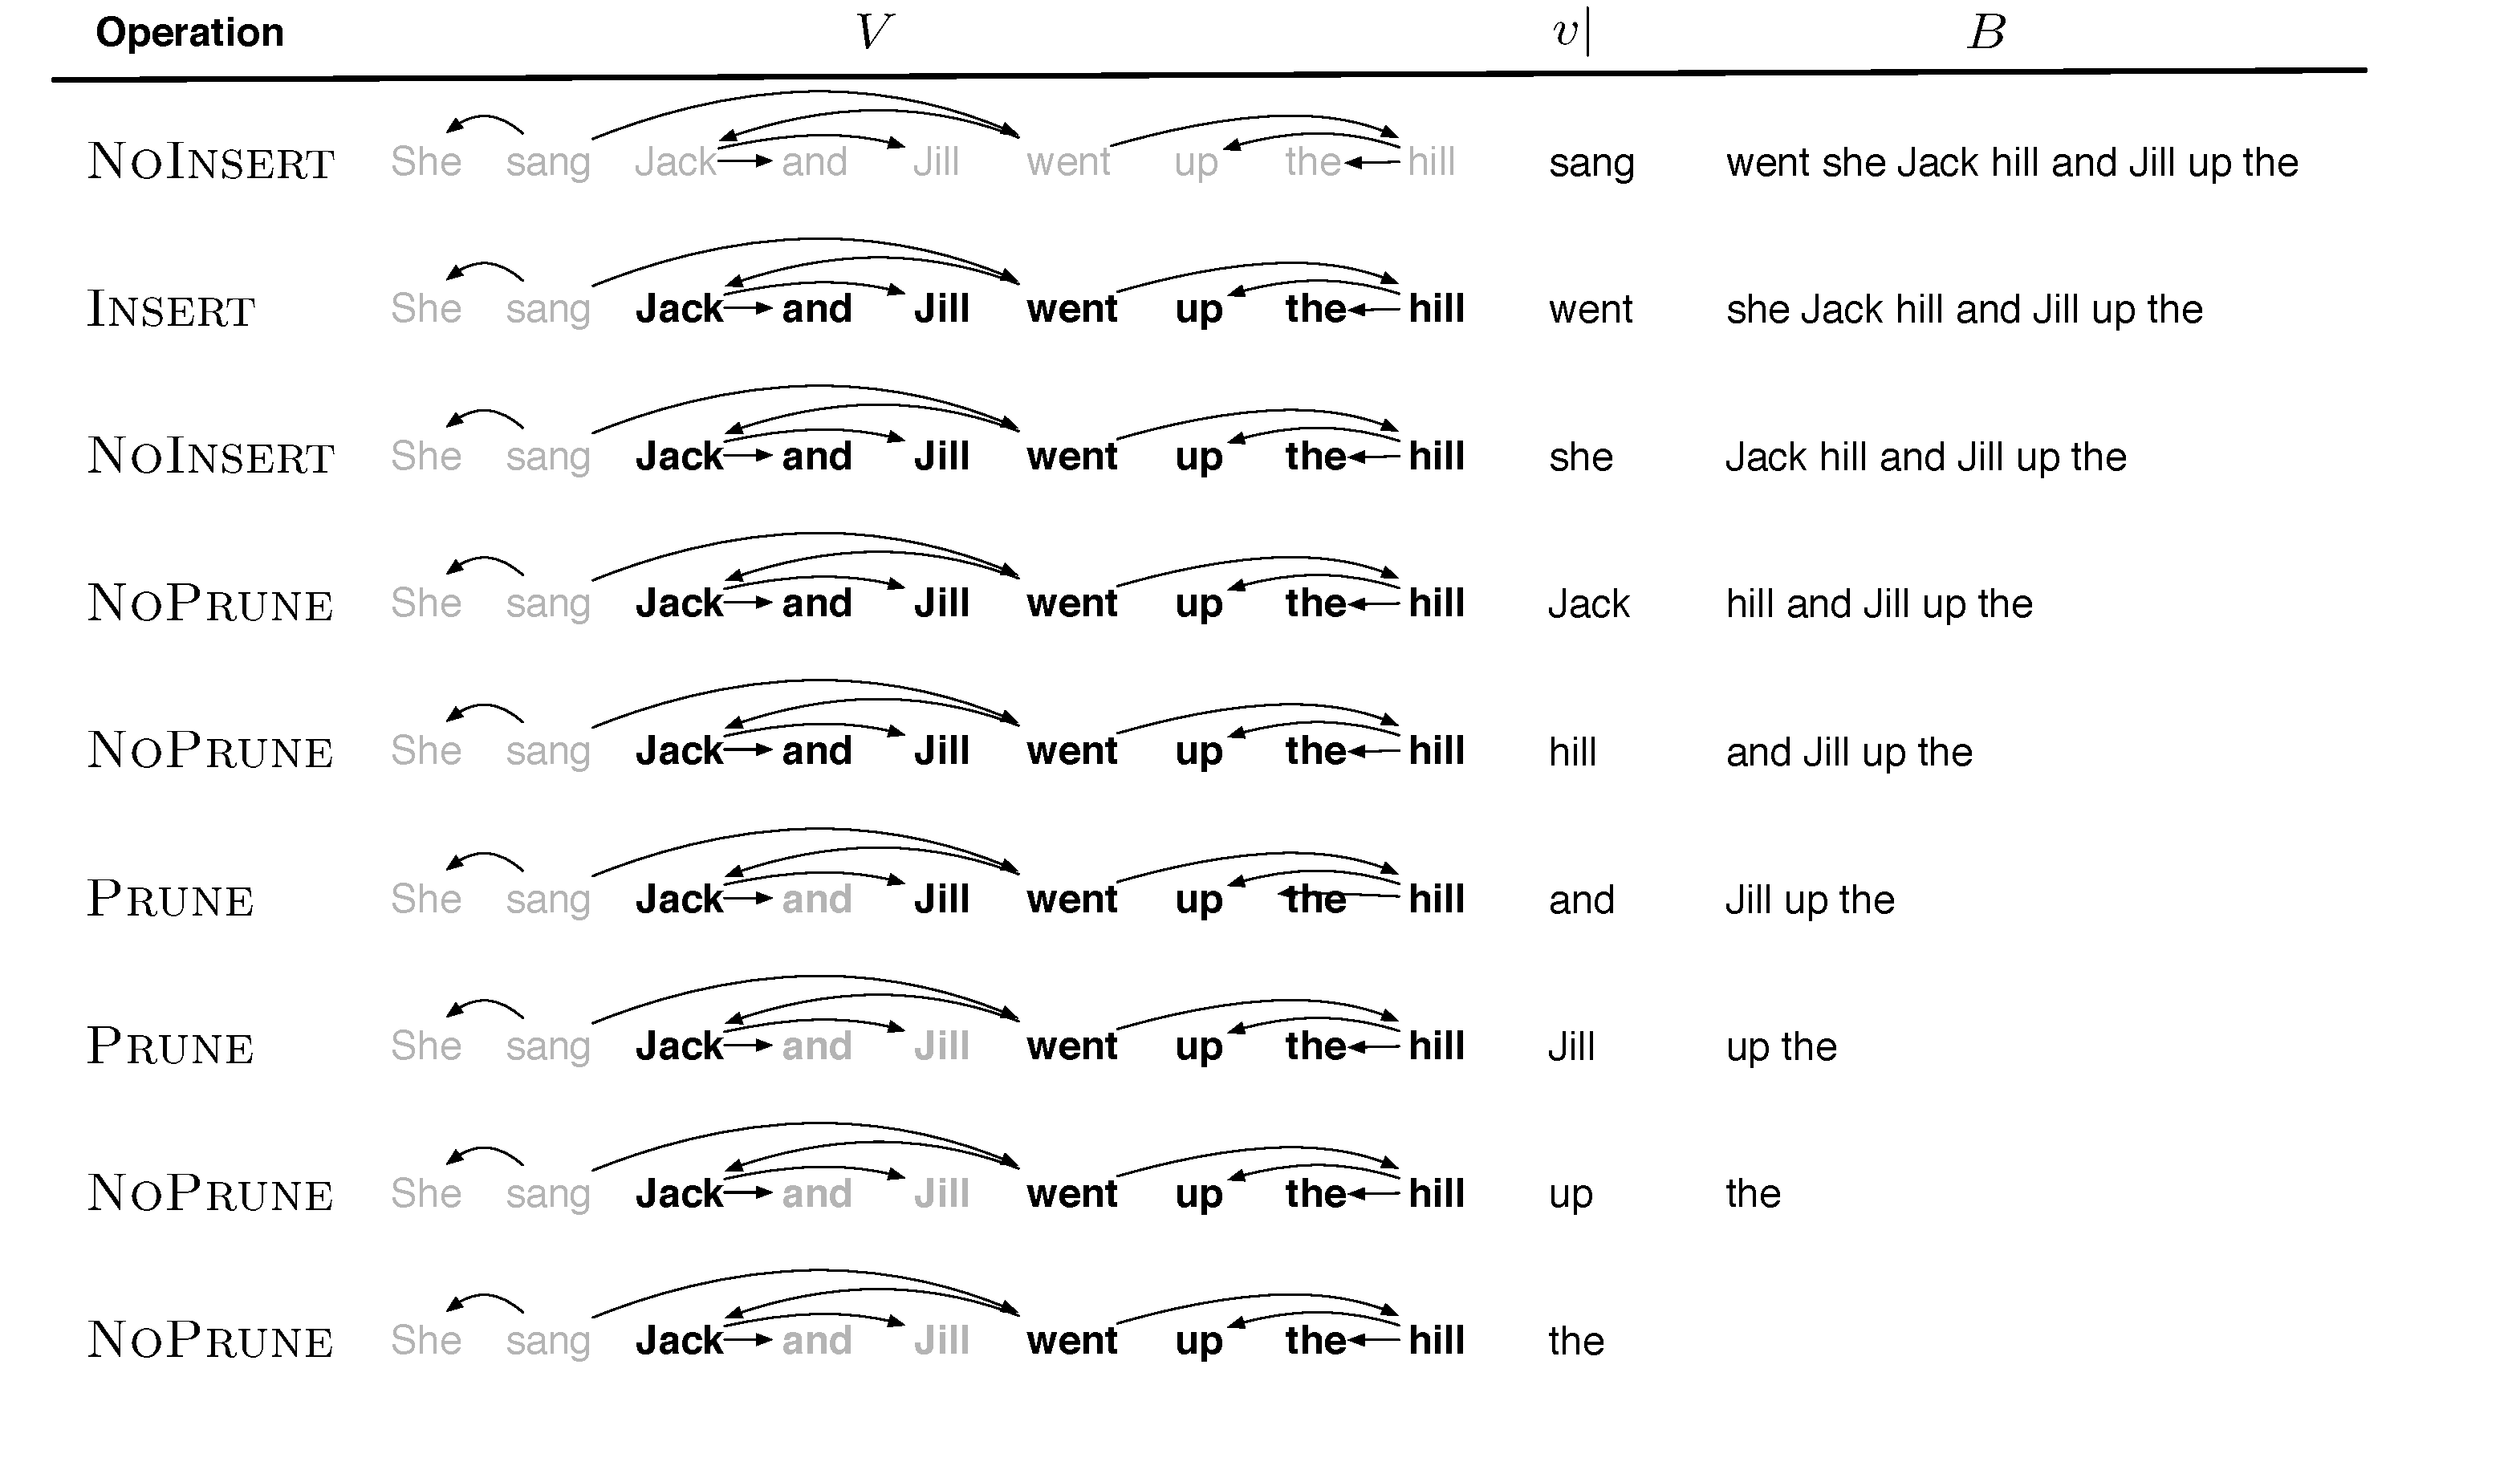
\includegraphics[width=.75\textwidth]{worked.pdf}
\caption{Nine operations of our transition-based compression return the compression: ``Jack went up the hill". At each timestep, the compression has state $(V, [v|B])$. In the diagram, the tokens in $V$ are shown in bold. At each timestep, the token $v$ at the head of the buffer $B$ is shown in the third column. Our compression system references the original, unchanging dependency parse of the sentence, $s$, shown in the diagram. The buffer is initialized breadth-first. Compression stops when the buffer is empty.}
\label{f:example}
\end{figure*}

Some discrepancies arise from differences in syntactic formalisms. To begin, prior work uses a tree transformation method which is no longer strictly compatible with UD. For instance, the tree transformation from prior work assumes PPs are headed by prepositions, which is not true in UD \cite{Schuster2016EnhancedEU}. In implementing the ILP, we use the enhanced dependencies representation from CoreNLP \cite{Schuster2016EnhancedEU}. The augmented modifiers and augmented conjuncts in this representation create parses that are very similar to the transformed trees described in prior work. \citet{filippova2008dependency} also describe a syntactic constraint based on the \rdep{sc} relation, which is not included in UD. We therefore exclude this constraint.

Other possible discrepancies arise from differences in part-of-speech taggers. In particular, prior work modifies a dependency tree by adding an edge between the root note and all verbs in a sentence, as a preprocessing step. This ensures that subclauses can be removed from parse trees, and then merged together to create a compression from different clauses of a sentence. However, we found that replicating this transform literally (i.e. only adding edges from the original root to all ``verbs'') made it impossible for the ILP to recreate some of the gold compressions in the dataset. (We suspect that this is because our part-of-speech tagger and the original part-of-speech tagger employed in \citet{filippova2013overcoming} sometimes return different part-of-speech tags). Our tree transform therefore adds an edge between the root node and \textit{all} tokens in a sentence. With this change, it is always possible for the ILP to output the gold compression.

We use \citet{gurobi} (v7) to solve the liner program. \citet{filippova2008dependency} report using LPsolve.\footnote{\url{http://
sourceforge.net/projects/lpsolve}}  We found that Gurobi sometimes segfaults nondeterminsitically during training. We implement checkpoints which save and restore the state of computation, allowing us to resume training when such errors occur. 

Lastly, in Table 1 of their original paper, \citet{filippova2013overcoming} provide an overview of the syntactic, structural, semantic and lexical features in their model. We implement every feature explicitly described in their work, except where otherwise noted (e.g. syntactic feature not compatible with UD). However, additional features implemented in their model (but not not described in their overview) almost certainly affect performance. 


\subsection{Implementation of SLOR: additional details}

We use the SLOR function to measure the readability of the shortened sentences produced by each compression system \ref{s:readabilityinformativeness}. Following \cite{lau2015unsupervised}, we define the function as 

\begin{equation}
\text{SLOR}=\frac{\text{log}P_m(\xi) - \text{log}P_u(\xi)}{|\xi|}
\end{equation}

where $\xi$ is a sequence of words, $P_u(\xi)$ is the unigram probability of this sequence of words and $P_m(\xi)$ is the probability of the sequence, assigned by a language model.  $|\xi|$ is the length (in tokens) of the sentence.

We use a 3-gram language model trained on the \citet{filippova2013overcoming} corpus. We implement with KenLM \cite{Heafield-kenlm}.

\subsection{Structure of subtree tags: additional details}\label{s:subtree}

Our markup input to our LSTM, $\bm{x}$, includes bracket symbols called \textit{subtree} tags with a complex structure, used to represent the start and end of the tokens which will be pruned or inserted by an operation $o \in \{ \textsc{Prune},\textsc{Insert}\}$. The start and end tags are each formed by concatenating two symbols: (1) a symbol $o$ indicating the type of the operation proposal (i.e. prune or insert) and (2) a symbol $d$ indicating the dependency type governing $T(v)$, such as \texttt{dobj}. 

\begin{table}[]
\begin{tabular}{@{}ll@{}}
\toprule
Batch size         & 135                      \\ \midrule
Hidden size        &                          \\
Embeddings dim.    & 300                      \\
Total fully-connected layers & 2                        \\
Fully-connected layers, hidden sizes & $(92, 2)$ \\
Fully-connected layers, dropout & $(0.3093, 0.4078)$ \\
Fully-connected layers, activations        & Relu, Linear             \\
Learning rate      & $4.593 * 10^{-4}$   \\
Weight decay       & $2.421 * 10^{-8}$   \\ \bottomrule
\end{tabular}
\caption{The hyperparameters for our model. We optimize hyperparameters via random search \cite{Bergstra2012RandomSF}. The learning rate and weight decay parameter each clearly affect validation accuracy. The importance of other parameters is less clear. } 
\end{table}



\bibliography{abe}
\bibliographystyle{acl_natbib}

\end{document}

%\ahcomment{Sort of hard to tell what formalism F and A use. I thnk it is stanford, but they don't come out and say it.They cite Nivre's book which references the malt parser which seems to use stanford deps. but I don't see mention of the ``in" relation referenced in F and A paper in a guide to stanford deps. Writing around it.}

% other ideas... 
 
%\section{Computational experiments part 2: investigating properties of q,s,r compression}

%\ahcomment{include?}

%\ahcomment{only outline / notes here}

%\begin{enumerate}
%\item{q = a list of 1 to 3 NER}
%\item{r = random}
%\item{What is the size of the minimum compression?}
%\item{Reachability by budget by position of q in syntax tree. (If q is more than one entity then how the entities are dispersed across the tree probably matters a bunch too).}%
%\item{Hang on. reachability == min compression, eh? if min compression $>$ b, it is clearly bad.}
%\item{Avoid computational waste w/ grammar.  Examine: ops you never have to worry about if you prune a branch v. dependency type deletion endorsement rate. Some ops get rid of lots of tokens w/ very high probability of deletion endorsements: e.g. parataxis (a great op!). By contrast: pruning a noun subj destroys acceptability and usually does not delete many tokens. Not worth the risk!}
%\item{What is the empirical number of ops (i.e. decisions you have to make about pruning) if you greedily drop branches but never drop if the single op probability is less than $p$? My guess is you can make this problem way, way, simpler than implied by exponential formulation. Is it really quadratic?}
%\item{Distribution of number of ops used for different q and r: when choosing ops at random? when choosing greedily? When pruning $\propto$ p(endorsement)?}
%\item{Other stuff: min compression, reachability, operations saved w/ big prunes? position of query in the tree?}
%\end{enumerate}
